\chapter{A PREDICTION OF THE THERMAL CONDUCTIVITY OF \ce{Au144PET60} NANOARRAYS}\label{chap:arrays}
\section{Introduction}
Thiolated gold nanocluster have been studied in great detail both experimentally and theoretically.\cite{Hakkinen2012, Sardar2009, Jin2010, Tsukuda2012}
The electronic,\cite{Lopez-Acevedo2011,Walter2008} optical,\cite{Cui2014} and catalytic properties;\cite{Chen2013, Lopez-Acevedo2010} promising to make them building blocks for nanotechnology applications.\cite{Dong2011,Podsiadlo2010,Shevchenko2006,Talapin2010}
These properties depend on sites of the particles, as well as the ligand identities.
Nanocrystal arrays, which are close-packed structures of nanoparticles in a colloidal solution, have been proposed as alternatives for more expensive single-cystal semiconductor materials in transistors,\cite{Talapin2005} memory devices,\cite{Sun1999} solar cells,\cite{Tang2011,Gur2005,Ehrler2012} and thermoelectrics.\cite{Ong:2013rt,Kovalenko2010,Wang2008,Ko2011} 

One of the first theoretical studies of nanocrystal arrays was performed by Luedtke and Landman.\cite{Luedtke1996}
They examined small clusters with alkanethiol ligands on a graphite surface and in superlattices. 
A more recent experimental study by Liu \textit{et al.} explored the effect of surface chemistry on the thermal conductivity of a nanocrystal array.\cite{Liu2015}
The study by Liu \textit{et al.} varied nanocrystal core size, the binding group of the ligand, and the ligand length. The primary finding was that with a decrease in ligand length or an increase in the core size, the thermal conductivity of the array increased.
The volume fraction of the insulating material (the ligand) is reduced in both of those cases.

Similar results with respect to the core diameter have been seen in theoretical studies of nanocrystal arrays by Ong \textit{et al.}\cite{Ong:2014yq} and Zanjani \textit{et al.}\cite{Zanjani2014} 
In particular Ong \textit{et al.} found that in nanocrystal arrays, vibrational states are able to elastically couple across the interfaces, yielding a thermal conductivity that is dependent on the density of the ligand layer.\cite{Ong:2014yq} The coupling was further studied by varying the core atomic mass and finding the relationship between core vibrational states and the interfacial thermal conductivity.

The study by Zanjani \textit{et al.} on gold nanocrystals with hexylthiol capping ligands varied both core size and ligand density.\cite{Zanjani2014}
The phonon dispersion of the superlattice structures was obtained and the thermal conductivity of the nanocrystal arrays displayed the same trends oberved by Liu \textit{et al.} that is, an increase in thermal conductivity of the array with decreased volume percentage of the ligand layer.\cite{Liu2015} 

All the nanoparticles previously studied contain less than 500 atoms. Recent work by Pohjolainen \textit{et al.} provides structures and force field parameters based upon crystal structures for thiolated gold nanoclusters found in a matching crystalography study of the clusters in arrays.\cite{Pohjolainen2016} 
These structures contain individual particles as well as nanoarrays, with the largest of the structures containing 144 \ce{Au} atoms. All of the characterized nanoclusters have a ``staple''-motif ligand that was shown to be thermally stable in this model. Many of the parameters were taken from work from Banerjee \textit{et al.} that explored \ce{Au25} and \ce{Au38} nanoclusters.

The staple motif in these nanoclusters presents an interesting test for theories of thermal transport. 
The staple motif has three gold atoms (for the largest particle), two of the gold atoms in the staple are in direct contact with the core of the particle, while the remaining atom resides in the ligand layer, but is bonded to sulfur atoms. In our previous work on the effect on thermal properties due to under-coordination of gold atoms the surface,\cite{Neidhart2017} the gold atoms within the staple motif may present interesting challenges. 
For this reason, we have looked at single particles and arrays of \ce{Au144PET60} clusters in two solvents, and look for agreement with the Hasselman and Johnson equation for thermal conductivity in composite materials.\cite{Hasselman}
\subsection{Theory}
Hasselman and Johnson first proposed a predictive formula for the effective thermal conductivity of a composite material using known bulk properties of the two complinents separately.\cite{Hasselman}
The original formulation of the Hasselman and Johnson equation for the effective thermal conductivity of the composite,
\begin{equation}
\label{eq:composite}
    \lambda_e = \lambda_s \bigg( \frac{\lambda_p (1+2\alpha)+2\lambda_s +2v_p[\lambda_p(1-\alpha)-\lambda_s]}{\lambda_p (1+2\alpha)+2\lambda_s -v_p[\lambda_p(1-\alpha)-\lambda_s]} \bigg)
\end{equation}
uses $\lambda_p$ and $\lambda_s$, the particle and solvent thermal conductivities, and $v_p$, the volume fraction of the nanoparticles. $\alpha$ is the interfacial term, which
is a dimensionless factor that relates the thermal boundary resistance to the radius of the particles.
The thermal boundary resistance in this work is
\begin{equation}
    \alpha = \frac{R_{TBR}}{r_p} = \frac{\lambda_s}{Gr_p}
\end{equation}
where $G$ is the interfacial thermal conductivity from the particle to the solvent, and $r_p$ is the radius of the particle.
Modifications to the Hasselman and Johnson equation have been made by Minnich \textit{et al.} to include an interface density for the spherical particles and a more formal volume fraction of the nanoparticles.\cite{Minnich2007}

Each portion of Eq. \ref{eq:composite} can be calculated separately in order to predict a composite material thermal conductivity. 
The volume fraction of the particles can be found through geometric means using the information about the particles in the array.
The thermal conductivity of the solvent, $\lambda_s$ , can be found through simulations of bulk solvent. 
Similarly, $\lambda_p$ can be calculated from bulk simulations of the core material of the particle. 
The most difficult piece to obtain is the $\alpha$ term, where the interfacial thermal conductance of the particles is the primary quantity of interest.
The interfacial thermal conductance of the nanoclusters investigated in this work were found using the same method as Stocker \textit{et al.} for nanospheres.\cite{Stocker2016}

Molecular modelling of heat conduction in nanoarrays considers only one method for thermal transport: conduction.
This work is a purely classical approximation of nanoarrays and does not consider electronic effects (such as polarization of the gold surface) or radiative transfer. 
While convection may be seen through classical simulations, it is not likely to be a large contribution to thermal transport in a densely-packed array. 
%Additionally, the solvent between the particles in the arrays could display altered diffusion coefficients due to confinement and change in temperature.
%Any coupling in these systems between the gold particles could only be seen through a classical means and the electronic contributions are not considered.
\section{Computational Details}
Nanoarrays of \ce{Au_144PET_60} solvated with either toluene or dichloromethane were simulated using reverse nonequilibrium molecular dynamics (RNEMD).
Individual components of these systems: e.g. single particles in each solvent, pure solvent, and liquid gold were also prepared and simulated using RNEMD.
The following sections describe the potentials used for the interactions in the system as well as how the systems were prepared.

\begin{figure}
    \centering
    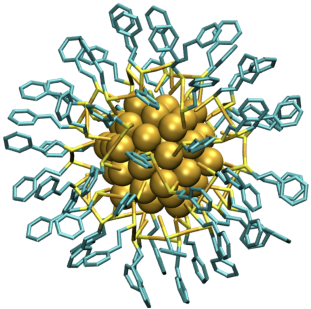
\includegraphics[scale=3]{figures/Au144-part.pdf}
    \caption{A single \ce{Au144PET60} cluster with the icosahedral core atoms rendered as spheres. All atoms in the ligand staple motof are displayed as stick like structures for clarity of the particle structure.}
    \label{fig:single-part}
\end{figure}

\subsection{Force Fields}
In the single particle systems and the liquid gold simulations, the gold--gold interactions are modeled using the quantum Sutton-Chen (QSC) potnetial.\cite{Qi:1999ph}
In the \ce{Au_144PET_60} particle, there are three distinct gold atom types: \ce{Au_{body}}, \ce{Au_{surface}}, and \ce{Au_{ligand}}. 
The gold interior to the particle, the icosahedral core, is defined as an \ce{Au_{body}} atom.
The other two gold atom types are part of the ligand staple motif and are directly bonded to sulfur atoms.
\ce{Au_{surface}} is the gold in the staple motif that is in direct contact with the surface of the particle. 
\ce{Au_{surface}} is treated with QSC for the interactions with \ce{Au_{body}} but with a Lennard-Jones potential for interactions with \ce{Au_{ligand}}, which is further from the surface of the particle and bonded between two sulfur atoms.
\ce{Au_{ligand}} is treated as a purely Lennard-Jones atom with parameters from Pohjolainen \textit{et. al.}.\cite{Pohjolainen2016}
All parameters for the staple motif use parameters from Pohjolainen \textit{et. al.}\cite{Pohjolainen2016} and Banerjee \textit{et al.}\cite{Banerjee2012} in addition to parameters from TraPPE-UA\cite{TraPPE-UA.alkanes,TraPPE-UA.alkylbenzenes} which can be found in Table \ref{tab:staple-parameters}.

\begin{figure}
    \centering
    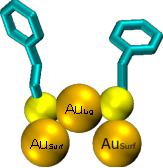
\includegraphics[scale=2]{figures/single.pdf}
    \caption{The \ce{Au} and \ce{S} atoms in the staple motif are depicted with spheres, while the \ce{PET} R groups are shown as stick like structures for clarity of the staple structure. The \ce{Au_{surf}} atoms sit directly on the icosahedral core of the nanocluster, while the \ce{Au_{lig}} atom is slightly out from the gold surface and are bonded to the sulfur atoms in two \ce{PET} ligands.}
    \label{fig:staple}
\end{figure}
\begin{landscape}
\begin{table}[]
\centering
\caption{Composition of a single nanoparticle and non-bonded interactions parameters for the interaction with gold. \label{tab:staple-parameters}}
\begin{tabular}{ c|ccccccl }
 \toprule
Sites & atoms & mass & $\sigma_{ii}$ & $\epsilon_{ii}$ & $\sigma_{\ce{Au}-i}$ & $\epsilon_{\ce{Au}-i}$  & source \\
     && (amu)& (\AA)        & (kcal/mol)     & (\AA)             &  (kcal/mol)          &  \\
\hline
 \ce{Au_{body}} &54&196.97&&\multicolumn{2}{c}{parameters from QSC}&\\
 \ce{Au_{surface}} &60&196.97&&\multicolumn{2}{c}{parameters from QSC}&\\
 \ce{Au_{ligand}} &30&196.97&2.629&5.2899&2.629&5.2899&Refs. \protect\cite{Pohjolainen2016} and \protect\cite{Banerjee2012}\\
 S           &60& 32.0655  & 4.45  & 0.2504 & 2.40   & 8.465  & Refs. \protect\cite{landman:1998} ($\sigma$) and \protect\cite{vlugt:cpc2007154} ($\epsilon$) \\
 \ce{CH2}    &120& 14.03    & 3.95  & 0.09141& 3.54   & 0.1749 & Refs. \protect\cite{TraPPE-UA.alkanes}, \protect\cite{vlugt:cpc2007154} and \protect\cite{landman:1998}\\
 CHar        &360& 13.02    & 3.695 & 0.1004 & 3.4625 & 0.1680 & Refs. \protect\cite{TraPPE-UA.alkylbenzenes} and \protect\cite{vlugt:cpc2007154}\\
 \bottomrule
\end{tabular}
\end{table}
\end{landscape}

To model solvents, dichloromethane and toluene, and the organic ligands, we use parameters from united atom models.
Dichloromethane is modeled with united atom Lennard-Jones atoms and charges taken from Meyer \textit{et. al.}\cite{Meyer1978} while the intramolecular parameters use harmonic force constants are adopted from OPLS-AA.\cite{Jorgensen98a}
Toluene is modeled as a rigid body using parameters from TraPPE-UA.\cite{TraPPE-UA.alkylbenzenes} %(From TraPPE-UA JPCB 104, 8008)
In the ligand staple motif, the carbon atoms were treated with TraPPE-UA,\cite{TraPPE-UA.alkanes,TraPPE-UA.alkylbenzenes,TraPPE-UA.thiols} while the sulfur parameters we adopted from TraPPE-UA\cite{TraPPE-UA.thiols} while bonds, bends, and torsions for the staple are adopted from Pohjolainen \textit{et al}.\cite{Pohjolainen2016}

Non-bonded interactions between the staple motif and icosahedral core of the particles are modeled using parameters derived from adsorption studies of thiolates on Au surfaces.
The S—-Au non-bonded parameters are adopted from work from Luedtke and Landman.\cite{landman:1998}

Other interactions between Au and non-metal atoms in the staple ligand are adapted from an adsorption study by Vlugt \textit{et. al.},\cite{vlugt:cpc2007154} of alkyl thiols on gold surfaces. The parameters are from a pair-wise Lennard-Jones potential for the interaction between Au and $\mathrm{CH}_x$ and S based upon the Hautman and Klein potential for Au(111) surfaces.\cite{hautman:4994}
The non-bonded interactions between gold atoms and toluene solvent use parameters from the same work.
Au and dichloromethane interactions use the aforemented work from Vlugt for the central carbon and the Au-Cl interactions through Johnson or Lorentz-Berthelot mixing rules.\cite{Johnson89}

\begin{table}
%\bibpunct{}{}{,}{n}{}{,}
\centering
\caption{Harmonic bond parameters for different components in the simulated systems. %The first part of the table are the atoms in the staple motif within the nanoparticle. The latter sections are the solvents: toluene and dichloromethane, respectively.
 \label{tab:abond}}
\begin{tabular}{ cc|ccl }
 \toprule
 $i$&$j$ & $r_0$ & $k_\mathrm{bond}$ & source \\
    &    & (\AA) & $(\mathrm{~kcal/mole/\AA}^2)$ & \\
\hline
\ce{Au$_{surf}$}   & \ce{S} &  2.41  &  150 & Ref. \protect\cite{Pohjolainen2016}\\
\ce{Au$_{lig}$}   & \ce{S} &  2.33  &  150 & Ref. \protect\cite{Pohjolainen2016}\\
S          & \ce{CH2} & 1.820   & 444  & Refs. \protect\cite{TraPPE-UA.thiols} and \protect\cite{Jorgensen:1996sf} \\
%\ce{CH3}   & \ce{CH2} & 1.540   & 536  & Refs. \protect\cite{TraPPE-UA.alkanes} and \protect\cite{Jorgensen:1996sf} \\
\ce{CH2}   & \ce{CH2} & 1.540   & 536  & Refs. \protect\cite{TraPPE-UA.alkanes} and \protect\cite{Jorgensen:1996sf} \\
CHar & \ce{CH2} & 1.540   & 536  & Refs. \protect\cite{TraPPE-UA.alkylbenzenes} and \protect\cite{Jorgensen:1996sf}\\
CHar       & CHar     & 1.40    & 938  & Refs. \protect\cite{TraPPE-UA.alkylbenzenes} and \protect\cite{Jorgensen:1996sf} \\
%\hline\hline
CHar       & CHar     & 1.40    & 938  & Refs. \protect\cite{TraPPE-UA.alkylbenzenes} and \protect\cite{Jorgensen:1996sf} \\
CHar       & \ce{CH3} & 1.540   & 536  & Refs. \protect\cite{TraPPE-UA.alkylbenzenes} and \protect\cite{Jorgensen:1996sf}\\
%\hline\hline
Cl      & \ce{CH2}   & 1.40    & 938  & Ref. \protect\cite{Meyer1978}\\
 \bottomrule
\end{tabular}
%\bibpunct{[}{]}{,}{n}{,}{,}
\end{table}

\begin{table}
%\bibpunct{}{}{,}{n}{,}{,}
\centering
\caption{Bend angle parameters for a harmonic potential. The central atom in the bend is atom $j$. 
%The table is structured with the particle staple motif in the first section, followed by the solvents: toluene and dichloromethane.
\label{tab:abend}}
\begin{tabular}{ ccc|ccl }
\toprule
 $i$&$j$&$k$ & $\theta_0$ & $k_\mathrm{bend}$ & source\\
    &   &    & ($\degree$) & (kcal/mol/rad\textsuperscript{2}) & \\
\hline
Au$_{surf}$ & S & Au$_{lig}$  & 91.3 & 460.24 & Ref. \protect\cite{Banerjee2012}\\
S& Au$_{lig}$ & S  & 172.24 & 240.24 & Ref. \protect\cite{Banerjee2012}\\
Au$_{surf}$ & S & \ce{CH2} & 111.6 & 146.37 & Ref. \protect\cite{Banerjee2012}\\
Au$_{lig}$ & S & \ce{CH2} & 106.8  & 146.37 & Ref. \protect\cite{Banerjee2012}\\
S & \ce{CH2} & \ce{CH2}& 114.0   &   124.20& Ref. \protect\cite{TraPPE-UA.thiols}\\
\ce{CH2} & \ce{CH2}  & CHar& 114.0   &   124.20& Ref. \protect\cite{TraPPE-UA.thiols}\\
\ce{CH2} & CHar     & CHar  & 120.0   &   140.0 & Refs. \protect\cite{TraPPE-UA.alkylbenzenes} and \protect\cite{Jorgensen:1996sf}\\
CHar     & CHar     & CHar      & 120.0   &   126.0 & Refs. \protect\cite{TraPPE-UA.alkylbenzenes} and \protect\cite{Jorgensen:1996sf}\\
%\hline \hline
\ce{CH3}     & CHar     & CHar  & 120.0   &   140.0 & Refs. \protect\cite{TraPPE-UA.alkylbenzenes} and \protect\cite{Jorgensen:1996sf}\\
%CHar     & CHar     & CHar      & 120.0   &   126.0 & Refs. \protect\cite{TraPPE-UA.alkylbenzenes} and \protect\cite{Jorgensen:1996sf}\\
%\hline\hline
Cl & \ce{CH2} & Cl & 111.8 & 155.39 &Ref. \protect\cite{Meyer96}\\
 \bottomrule
\end{tabular}
%\bibpunct{[}{]}{,}{n}{,}{,}
\end{table}

\subsection{Simulation Protocol}
The gold particle simulations are started from crystal structures provided in work from Pohjolainen \textit{et. al}.\cite{Pohjolainen2016}
The crystal structures were thermalized to 250K then solvated using Packmol\cite{packmol} with either dichloromethane or toluene molecules that were also equilibrated to 250K.
The solvent sphere was created to be at least 3x the radius of the particle with the solvent maintaining bulk density near the interface (see Table \ref{tab:solvated-part-comp} for exact packing).
At least 7 separate statistically independent configurations of the nanoparticles were created.

Solvated particles were then brought to 250K using the Langevin Hull ensemble.\cite{Vardeman2011} 
Once equilibrated with thermal coupling to the bath for at least 1 ns, the system was simulated without coupling to the bath for 1 ns. 
The particles were then simulated using RNEMD for 1 ns where a thermal flux was applied to create a radially-decaying temperature gradient. 
\begin{figure}
    \centering
    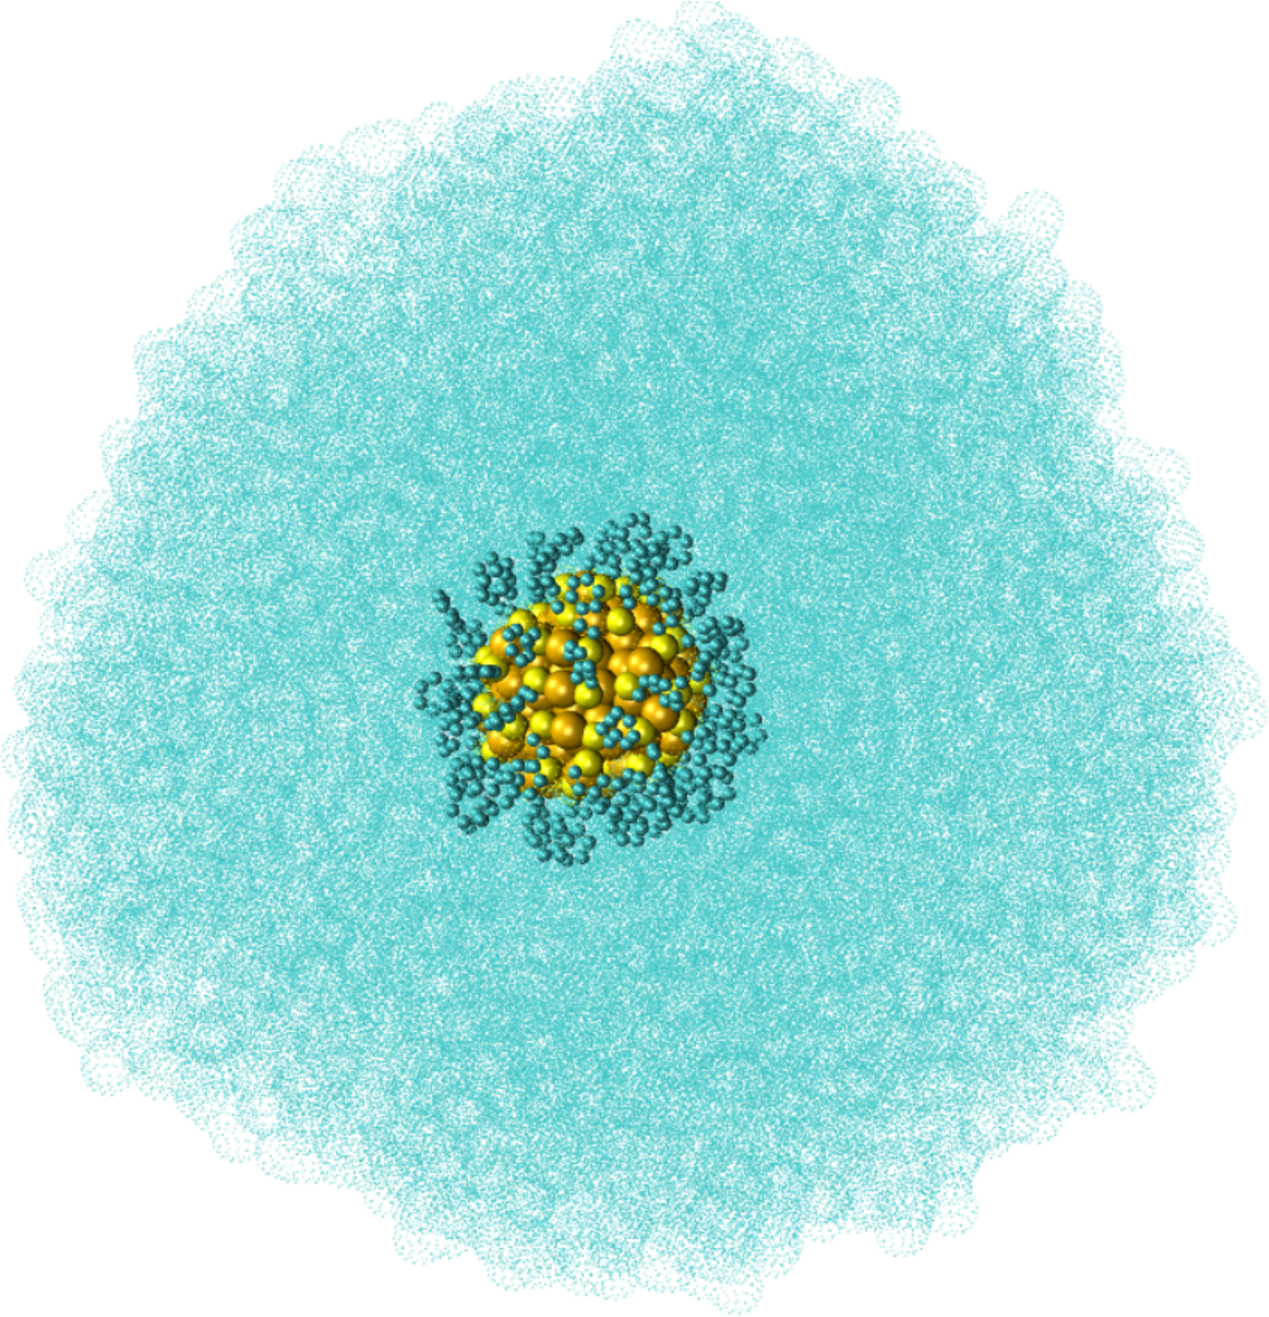
\includegraphics[scale=0.4]{figures/dcm-part.pdf}
    \caption{ A single \ce{Au144PET60} cluster in a solvent cloud of dichloromethane.}
    \label{fig:lambda-bulk}
\end{figure}

Pure solvent simulations were prepared using the bulk solvent density. 
Five statistically independent simulations for each of the three different simulation box lengths.
These simulations were equilibrated to 250K using the canonical (NVT) ensemble for at least 1 ns followed by further relaxation in the (NPT) ensemble for 1 ns.
Finally, the pure solvent systems were equilibrated for at least 1 ns in the microcanonical (NVE) ensemble before undergoing a 10 ns RNEMD simulation.

The pure gold systems followed the same protocol as the dichloromethane and toluene systems, except the temperature for the pure gold system is 1500K, above the melting point of bulk gold.
After equilibration, the relevant thermal flux was applied for 3 ns.
To achieve a similar temperature gradient across the three box sizes (for all bulk simulations), the applied thermal flux was adjusted, see Table \ref{tab:bulk-comp}.
Depending on the size of the simulation box, longer times are needed to allow a steady state temperature gradient to develop, so all systems were run for the duration needed to achieve this steady state.

The average temperature of the system remained at 250K for the pure solvent, single nanoparticle, and nanoarray systems; and 1500K for the liquid gold simulations.
In the pure solvent, single nanoparticle, and nanoarray systems this temperature preserved the solvent cloud close to the bulk density near the interface of the particle.
Additionally, thermal coupling to the external temperature bath for the single nanoparticle systems was removed to avoid thermal interference with the imposed flux.

%For the pure solvent and gold simulations, 15 independent simulations were carried out with five systems with random seeds at three different box lengths.
%The single nanoparticle simulations use at least 7 separate configurations of the nanoparticles before the random packing of each solvent, to ensure statistical independence.

\begin{landscape}
\begin{table}[]
    \centering
    \caption{Composition of the pure liquid simulations with box dimensions and average $\lambda$ values with standard error from 5 simulations.}
    \begin{tabular}{c|c|ccc|c|c|c}
    \toprule
         System& molecules & L$_x$ (\AA\ )&L$_y$ (\AA\ )&L$_z$ (\AA\ )& applied flux& run time&$\lambda$ \\
	& \multicolumn{3}{box dimensions} & units & (ns) & W/mK\\
         \hline
         Dichloromethane&2816&60.16&60.16&82.73&1E-7&10&0.0263 $\pm$ 7.0x10-4\\
         &5632&60.16&60.16&169.1&5E-8&10&0.0390 $\pm$ 2.0E-3\\
         &8448&60.16&60.16&253.35&5E-8&10&0.0595 $\pm$ 4.6E-3\\
         Toluene& 1764&62.3&62.3&80.1&1E-7&10&0.1036 $\pm$ 4.0E-3\\
          &3528&62.3&62.3&160.2&5E-8&10&0.1147 $\pm$ 1.0E-2\\
          &5292&62.3&62.3&240.5&5E-8&10&0.1062 $\pm$ 6.3E-3\\
         Gold& 5040&32.03&30.82&106.4&6.5E-6&3&0.3407 $\pm$1.0E-2\\
          & 10080&32.03&30.82&212.8&6.5E-6&3&0.3800 $\pm$ 1.9E-2\\
           & 15120&32.03&30.82&319.26&6.5E-6&3&0.3645 $\pm$ 2.0E-2\\
         \bottomrule
    \end{tabular}
    \label{tab:bulk-comp}
\end{table}
\end{landscape}

\begin{table}[]
    \centering
    \caption{Composition of solvated nanoparticles for interfacial thermal conductivity simulations.}
    \begin{tabular}{c|c|c}
    \toprule
         &Dichloromethane  & Toluene\\
         \hline
         atoms& 4807 &12075\\
         packing radius (\AA )& 52 &85\\
         average $\rho_{sim}^{r>20\AA}$  ($g/cm^3$)& 1.33 &1.74\\
         $\rho_{solv}^{bulk}$  ($g/cm^3$)& 1.33&0.87\\
    \bottomrule     
    \end{tabular}
    \label{tab:solvated-part-comp}
\end{table}

\begin{table}[]
    \centering
    \caption{Composition of nanoarray systems.}
    \begin{tabular}{c|c|c|c|ccc}
    \toprule
         System& \ce{Au144PET60} &DCM& Toluene& L$_x$ (\AA\ )&L$_y$ (\AA\ )&L$_z$ (\AA\ ) \\
         \hline
         2x2x2& 8&1100&450&61&61&61\\
         2x2x4& 16&2200&900&61&61&122\\
         2x2x6& 24&3300&1350&61&61&183\\
         2x2x8& 32&4400&1800&61&61&244\\
         \bottomrule
    \end{tabular}
    \label{tab:my_label}
\end{table}

The nanoarrays were construced using eight different particle geometries, packed in a 2 x 2 x 2 array, with a center of mass to center of mass distance of 30 \AA.
These arrays were thermalized to 250K, then solvated with either toluene or dichloromethane with random seeds to create five different configurations of the solvent.\cite{packmol}
Solvated arrays were equilibrated at 250K in the canonical ensemble then further equilibrated for at least 1 ns in the microcanonical ensemble.
These simple structures were replicated in the z-direction to create multiples of the unit cell, up to a 2x2x8 particle array, then equilibrated at 250K in the canonical ensemble and at least 1 ns in the microcanonical ensemble.

After equilibration the arrays were simulated with a thermal flux for at least 10 ns or until a steady state was reached.
To achieve similar temperature gradients across the box, the applied thermal flux was adjusted for the different array sizes.

All simulations were carried out using the open source molecular dynamics package OpenMD.\cite{openmd}
Thermal conductivity and interfacial thermal conductivity were calculated using methods described in works by Kuang \textit{et. al.} for periodic systems,\cite{Kuang:2011ef} and Stocker \textit{et. al.}  for non-periodic systems.\cite{Stocker:2014qq}

\subsection{Calculating thermal conductivity}
Under a linear response, the thermal conductivity is related to the applied flux,
% through the following:
\begin{equation}
    J_z = \lambda \Big\frac{\partial T}{\partial z}(\Big)	
    %\lambda = \frac{J_z}{\frac{\partial T}{\partial z}} = \frac{J_z}{m}
\end{equation}
where $J_z$ is the applied thermal flux and $\frac{\partial T}{\partial z}$ is the temperature gradient that develops in the simulation.
The thermal gradient created from the applied flux in a box of solvent is shown in Fig. \ref{fig:lambda-grad}. The red and blue bins are the hot and cold RNEMD exchange regions, respectively.
%The slope of the temperature gradient, $m$, is $\frac{\partial T}{\partial z}$.

\begin{figure}
    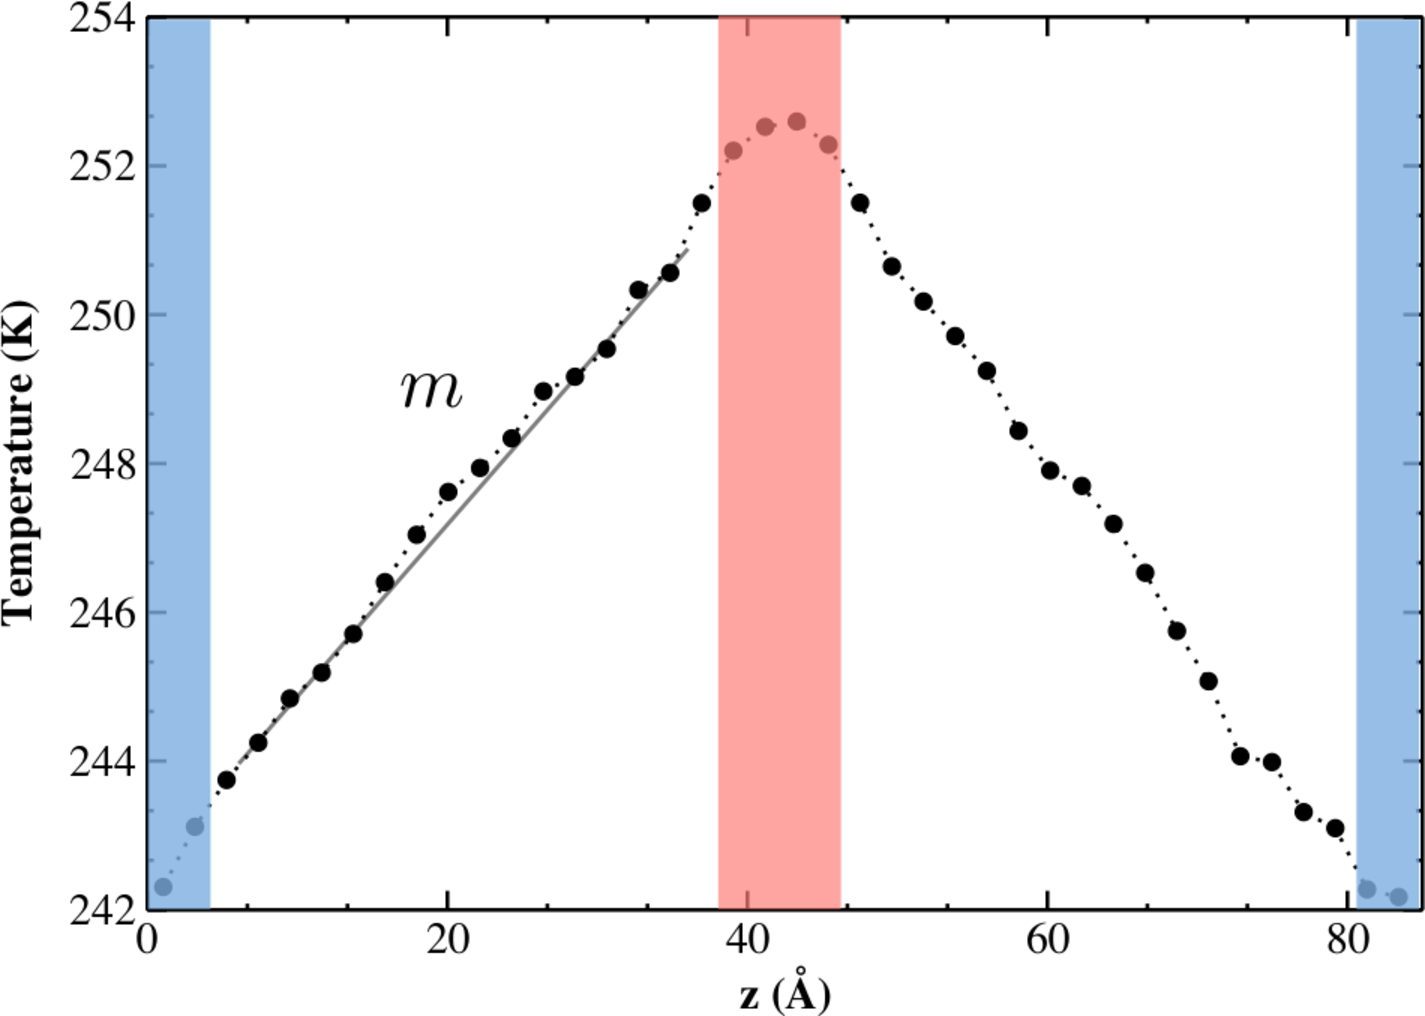
\includegraphics[scale=0.6]{figures/bulk-gradient.pdf}
    \caption{This figure is an example of the thermal gradient that develops in a bulk solvent system with a moderate flux. The red region is the ``hot'' bin and the two blue regions are the ``cold'' bins. The slope, $m$, that measures the temperature gradient is related to the thermal conductivity of the material, $\lambda$.}
    \label{fig:lambda-grad}
\end{figure}

In addition to finding the thermal conductivity of a material at different box lengths, the infinite box thermal conductivity of the material is extrapolated using the following equation:
\begin{equation}
    \frac{1}{\lambda_{\infty}}= \frac{1}{\lambda_L} +\frac{C}{L}
    \label{eq:lambda_inf}
\end{equation}
where $C$ is a constant and $L$ is the length of the simulation box in the z-direction.\cite{Hannah2015} 

\section{Results and Discussion}
A prediction using Eq. \ref{eq:composite} for a simple array of \ce{Au144PET60} particles can be made using separate simulations of each of the components of the system.
The bulk gold conductivity is compared to a previous study looking at gold particles in an array. 
Ultimately, as found in previous work by Zanjani \textit{et al.}\cite{Zanjani2014} and Ong \textit{et al.}\cite{Ong:2014yq}, the volume fraction of the array occupied by the particles is the essential piece of the predictive equation.
While the interfacial details is of lesser importance to the prediction of the thermal conductivity of the material, the two solvents do alter heat transport out of the nanoclusters.
This confirms previous findings regarding solvent penetration being paramount to thermal transport.
In the following sections, each of the individual components of the Hasselman and Johnson equation, as well as the overall prediction will be presented.
Additionally, thermal conductivity of the arrays will be discussed in comparison to the predicted results.

\subsection{Bulk Solvent and Bulk Gold Conductivity}
For the bulk dichloromethane and toluene solvent simulations, both were projected to infinite system size thermal conductivity using Eq \ref{eq:lambda_inf}. 
As seen in Fig. \ref{fig:inverselambda}, the box length projections of thermal conductivity is necessary for the dichloromethane solvent.
While projection to an infinite box size using Eq. \ref{eq:lambda_inf} is not required by the data for toluene and liquid gold.

The thermal conductivity of the dichloromethane from the projection to an infinite box and the thermal conductivity average of the toluene boxes are shown in Fig. \ref{fig:lambda-bulk}.
The infite box thermal conductivity of dichloromethane is 0.1084 $\pm$ 0.0021 W/mK and the conductivity of toluene is averaged to be 0.1082 $\pm$ 0.0054 W/mK.
If composition of the array is primarily solvent, the Hasselman and Johnson equation will therefor give nearly the same conductivity for the arrays.
It is important to note that the applied flux was small enough so that the density of the solvent across the simulation box was uniform.

\begin{figure}[h]
    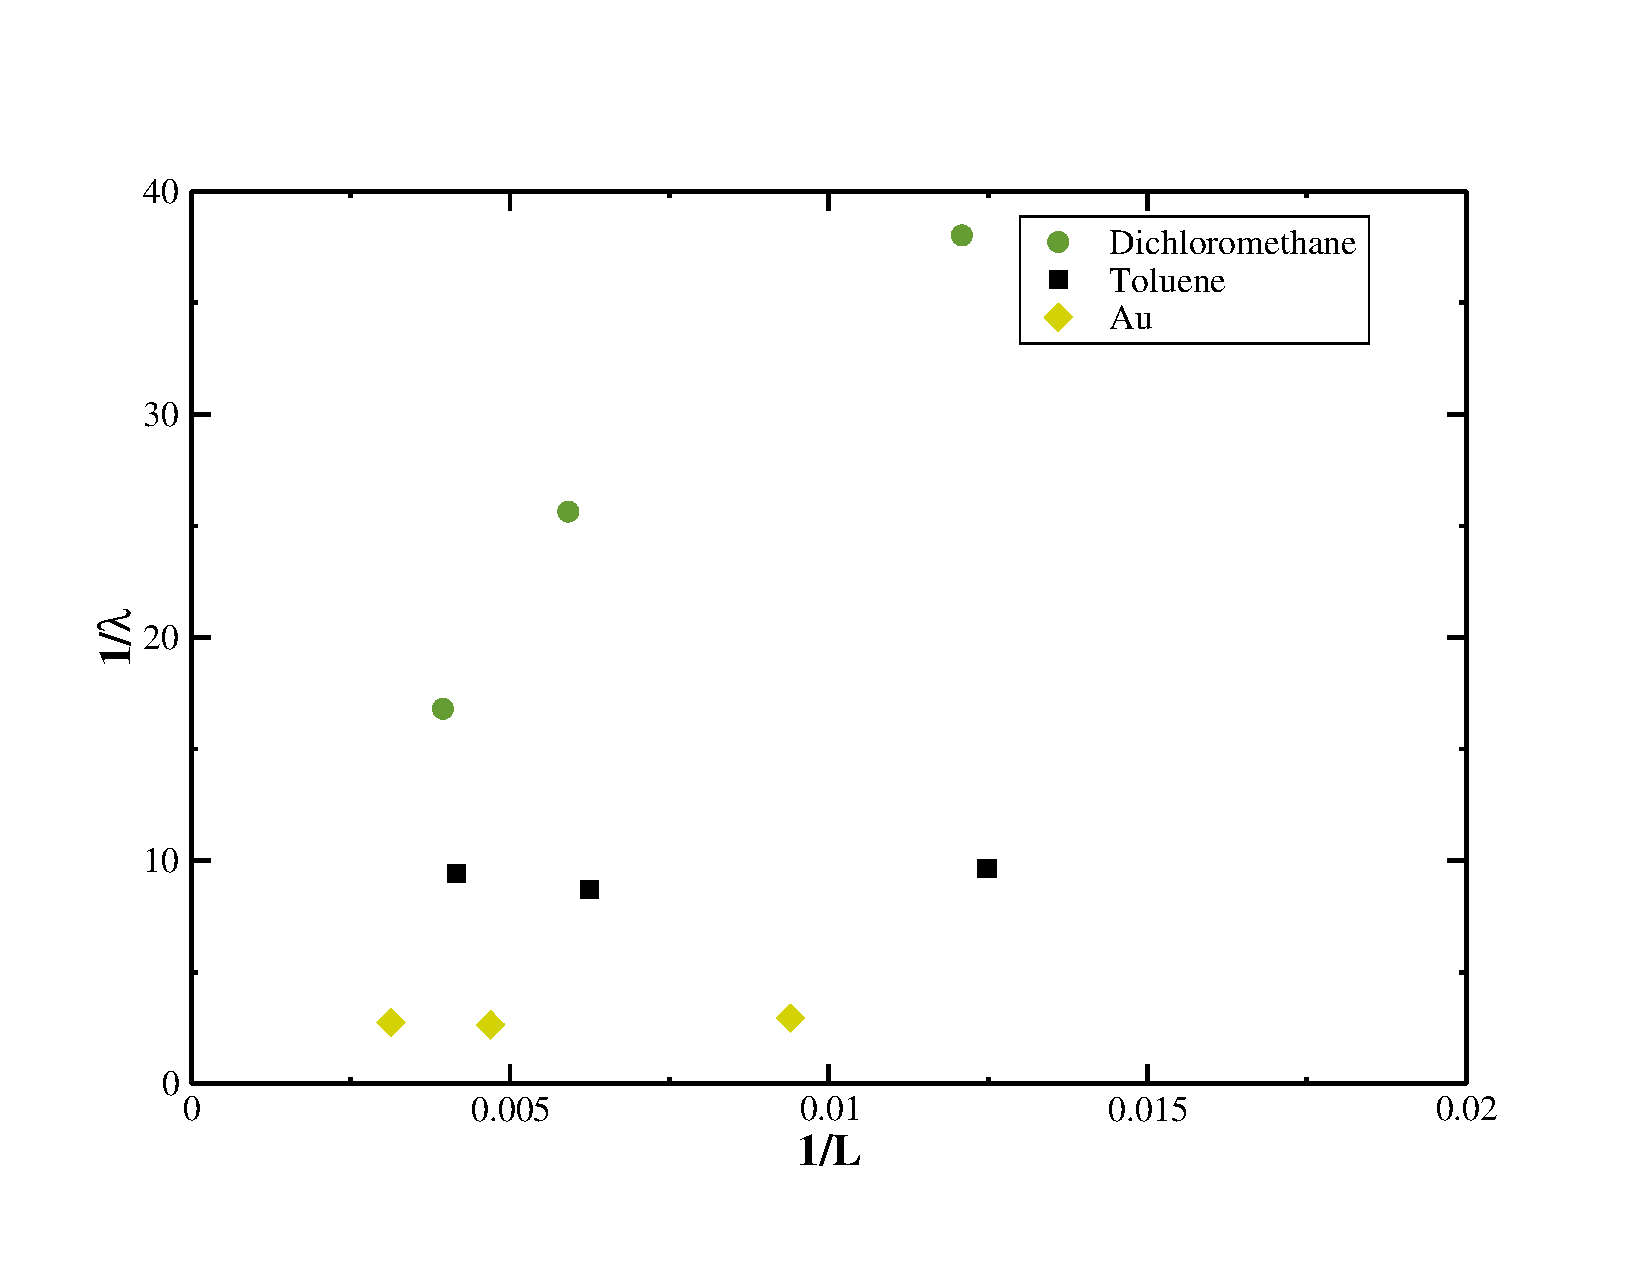
\includegraphics[scale=0.5]{figures/inverselambda-solvent.pdf}
    \caption{ Parameters to Eq. \ref{eq:lambda_inf} for bulk simulations of dichloromethane (green circles), toluene (black squares), and liquid gold (yellow diamonds). The y-axis, $\lambda$ is in units of W/mK. The x-axis, $L$ is in \AA.}
    \label{fig:inverselambda}
\end{figure}

%\begin{figure}[h]
%    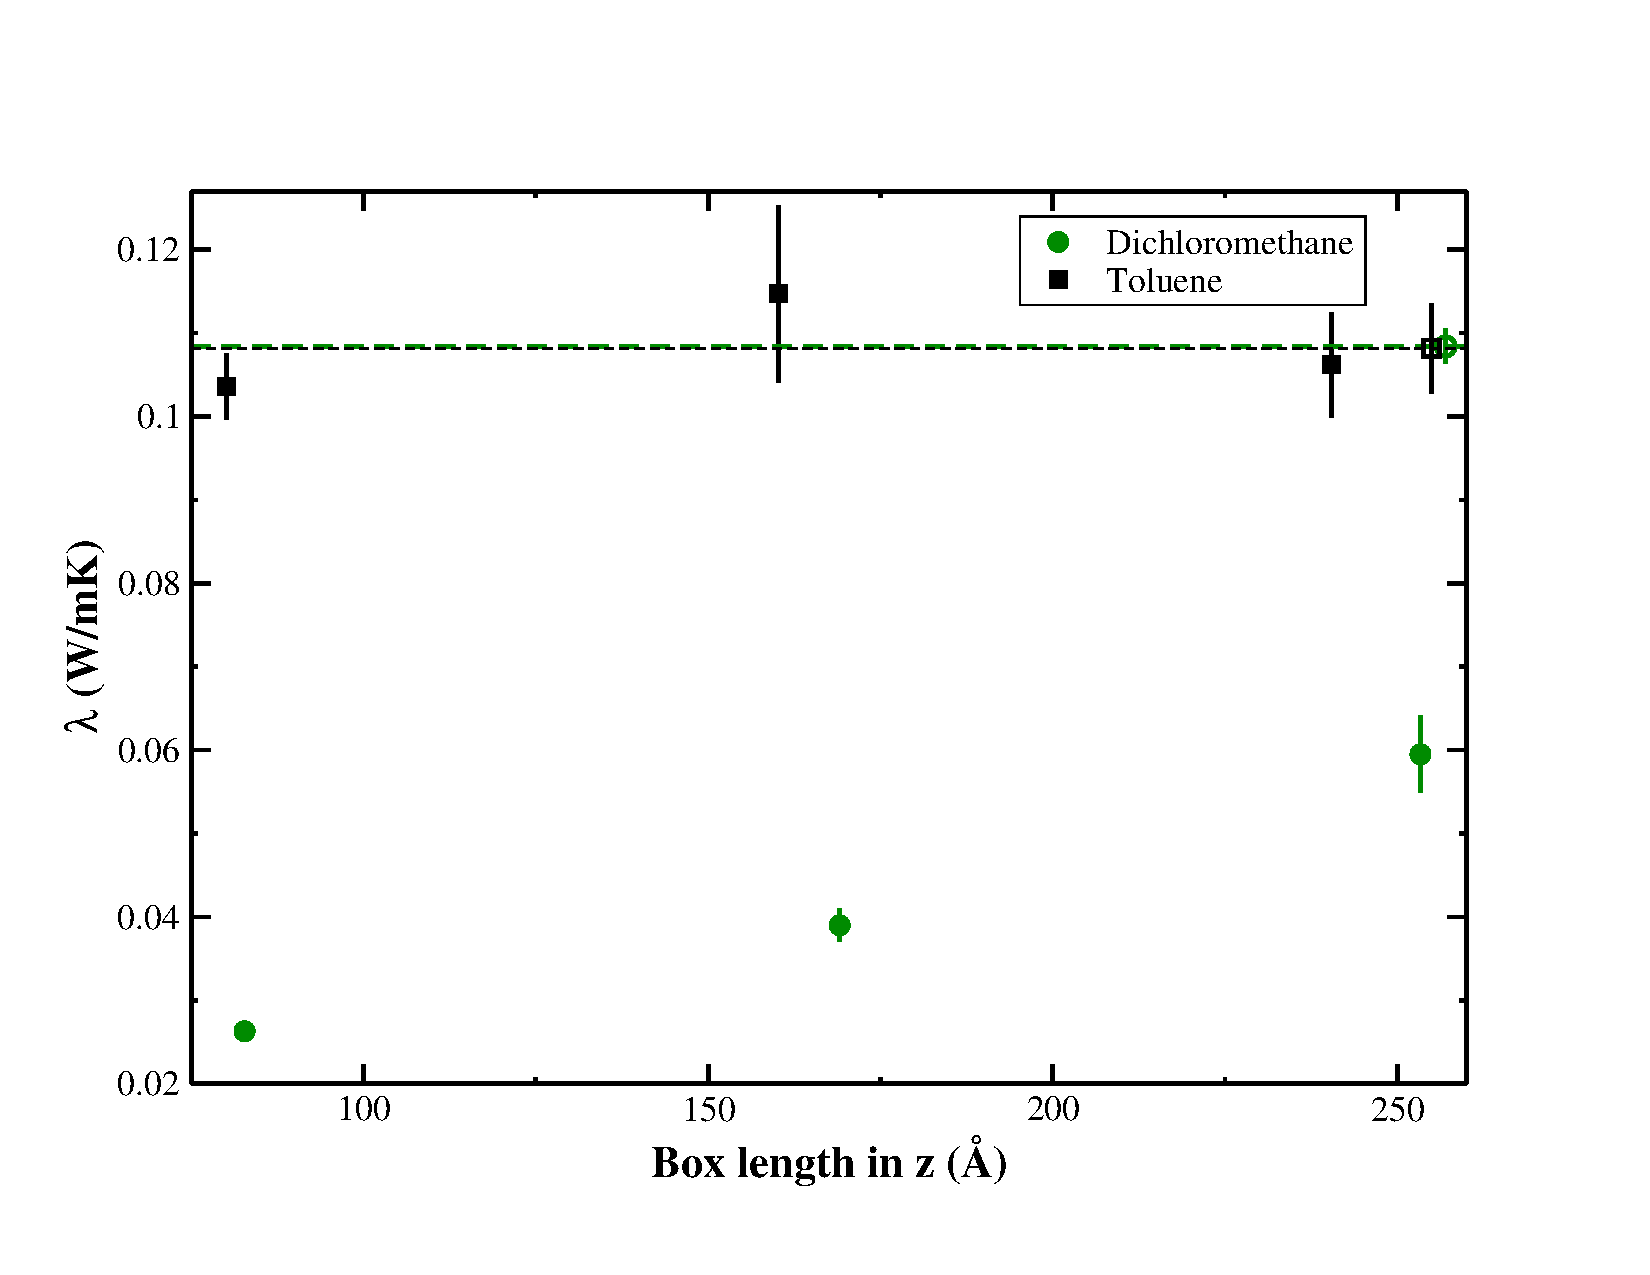
\includegraphics[scale=0.5]{figures/lambda-bulk.pdf}
%    \caption{ Bulk solvent $\lambda$ as a function of simulation box length in z displays the trend in dichloromethane with increasing box size. The dashed lines and open symbols are the projected $\lambda_{\infty}$ for dichloromethane and the average value for toluene.}
%    \label{fig:lambda-bulk}
%\end{figure}

The bulk gold simulations are essential to finding $\lambda_p$. Previous work from Ong \textit{et al.}\cite{Ong:2014yq} used bulk gold thermal conductivity of 1.8 $\pm$ 0.3 W/mK from simulations of a bulk `fcc' gold at 300 K for simulations of a gold nanocrystal array.
Their value will be compared to the conductivity of a bulk gold simulation at 1500 K, pass the melting point of the gold in QSC.
QSC has a size dependent melting temperature and previous particles of slightly larger radius have been shown to display liquid like structures.\cite{Stocker2016}
Experimentally, particles with $N<219$ have been seen with an approximate melting temperature of 500 K.\cite{Ercolessi1991}
Additionally, it was proposed through extrapolating melting temperatures vs. diameter, that the \ce{Au144PET60} cluster (with a diameter of $\approx$ 18 \AA) would melt at approximately 600 K.\cite{Buffat1976}
Hence the high temperature simulations of 100 \AA, 200 \AA, and 300 \AA\ box length in z were computed and displayed $\lambda_p$ = 0.3787 $\pm$ 0.02 W/mK.
The lower conductivity makes some sense; when the gold melts, the ballistic phonons traveling through the gold lattice are disrupted, and the transmission of the phonons decreases.

\subsection{Interfacial Thermal Conductivity}
The interfacial thermal conductance, $G$, for the particles was found in both solvents.
%In an attempt to force the interfacial density of toluene in these single particle to more closely match the experimental bulk density, 
The solvent outside of the interfacial region of the system is about twice the density of bulk toluene to maintain the solvent near the interface at a normal density.
This was not an issue with the dichloromethane systems. 
Across the staple motif the thermal conductivity to the toluene was 11.37 $\pm$ 0.66 MW/m$^2$K, while to dichloromethane $G$ = 74.73 $\pm$ 4.28 MW/m$^2$K.

%POSSIBLY SOMETHING ABOUT THE INTERPENETRATION OF SOLVENT
\subsection{Prediction of Array Thermal Conductivity}
Along with the components of the equation for bulk thermal conductivity, $v_p$, the partial volume of the \ce{Au144PET60} particles in the array is required to predict array conductivity.
The partial volume is approximated through the effective radius of the particles, which is taken from the average of the radius for only the outermost gold atoms and the radius of the total particle including the staple motif.
This approximations gives a partial volume of 22.5\%.
A total particle volume which includes all the ligand layer, allows for solvent to penetrate into the particle and would overestimate the volume fraction of the particles for a $v_p = 47.7\%$.

Using the parameters calculated in this study, $\lambda_s$, $\lambda_p$, $G$, and $v_p$, Eq.\ref{eq:composite} used to predict the thermal conductivity of the array.
Using the bulk gold thermal conductivity reported by Ong \textit{et al.} for gold at 300 K and the value calculated here for 1500 K, the array thermal conductivity can be found in Table \ref{tab:predition}.
As seen in previous work,\cite{Ong:2014yq, Liu2015, Zanjani2014} the volume fraction of the particles is the main determining factor of the thermal conductivity. 
With the small $v_p$, $\lambda_s$ dominates $\lambda_e$, thus there is a similar conductivity for the array across solvent (since $\lambda_s$ is nearly the same for the bulk thermal conductivity) and $\lambda_p$.

\begin{table}[]
    \centering
    \begin{tabular}{c|c|c}
    \toprule
         &$\lambda_p^{1500 K}$ & $\lambda_p^{300 K}$  \\
         \hline
         $\lambda_e^{DCM}$& 0.1184& 0.1256\\
         $\lambda_e^{Toluene}$ & 0.1182 & 0.1254 \\
         \bottomrule
    \end{tabular}
    \caption{The Hasselman and Johnson prediction for thermal conductivity of the \ce{Au144PET60} array using the gold thermal conductivity at 1500 K and 300 K. The array prediction for dichloromethane and toluene using the bulk thermal conductivity of each solvent.}
    \label{tab:predition}
\end{table}

\subsection{Simulations of Arrays}
Preliminary results of the smallest arrays displays behavior that indicate that Eq. \ref{eq:composite} might be missing a more complex component of the system.
The smallest system (2x2x2) in dichloromethane was simulated to find $\lambda = 0.0307 \pm 0.009$ W/mK. 
This is far below the predicted value of 0.1184 W/mK, but the dichloromethane bulk solvent displayed length-dependent thermal conductivity.
Therefore, it is possible that with larger arrays in dichloromethane, a length-dependent thermal conductivity will be extrapolated. 
Additionally, it is possible that the dichloromethane in the arrays behaves differently than the bulk fluid and might have thermal properties more similar to a confined liquid.

\section{Conclusions}
While there is still more that needs to be explained in the nanoarrays of the \ce{Au144PET60} particles, interesting results have been found using the Hasselman and Johnson model. 
To use the model, each component of the nanoarray was simulated to find the relevant thermal transport property. 
As found in previous works, the main component of the Eq. \ref{eq:composite} is $v_p$. 
The geometric arrangement of the array is the most important aspect contributing to the thermal conductance of the material.

In finding the component pieces of Eq. \ref{eq:composite}, interest results were found for the pure liquid simulations and the interfacial thermal conductivity of the particle.
The two solvents do not have the same length-dependent behavior thermal transport properties. This suggests interesting differences for the density dependent thermal conductivity in liquids.
Similarly, the large difference in $G$ between the two solvent interfaces with the particle, brings about questions of what is most important in ligand--solvent design.
